% a-project.tex, v-1.0.3 marcoreis baseado no
% abntex2-modelo-trabalho-academico.tex, v-1.9.7 laurocesar
% Copyright 2012-2018 by abnTeX2 group at http://www.abntex.net.br/ 
% 
% This work consists of the files 
% 
% -----------------------------------------------------------------------------
% Modelo para desenvolvimento de documentação de projetos acadêmicos
% (tese de doutorado, dissertação de mestrado e trabalhos de monografias em geral) 
% em conformidade com ABNT NBR 14724:2011: Informação e documentação. 
% -----------------------------------------------------------------------------
% Opções para a documentação
%
% Fancy page headings 
%\documentclass[fancyheadings, subook]{Classes/a-prj}
%\documentclass[fancyheadings, sureport]{Classes/a-prj}
%
% Fancy chapters and sections headings 
%\documentclass[fancychapter, subook]{Classes/a-prj}
%\documentclass[fancychapter, sureport]{Classes/a-prj}
%
% Fancy page , chapters and sections headings
%\documentclass[fancyheadings, fancychapter, subook]{Classes/a-prj}
\documentclass[fancyheadings, fancychapter, sureport]{Classes/a-report}
%
% -----------------------------------------------------------------------------
% Alguns comandos para a fancy page headings)
%
% Page header line width
%\footlinewidth{value}
%
% Page footer line width
%\headlinewidth{value}
%
% Page header and footer line width
%\headingslinewidth{value}
%
% Page header and footer lines without text
%\headingslinesonly
%
% The default line width is 0.3pt.
% Set the value to 0pt to remove the page header and/or footer line
%
% -------------------------------------------------------------------------------
% Formato de figuras suportado
% -------------------------------------------------------------------------------
% O formato das figuras depende da forma como o arquivo de saída é gerado.
% As figuras inseridas na pasta Figures serão automaticamente reconhecidas sem
% a necessidade de inserir a extensão do arquivo.
%
% O pdfLaTEX (PDF) suporta figuras com as extensões: pdf, jpg, png e mps.
%
% -------------------------------------------------------------------------------
% Árvore do diretório a-project.tex
%  Diretório
%       \Classes        (requerido)
%       \Figures        (requerido) --------------------------------->
%       \Figures\PDF    (optional)
%       \Figures\JPG    (optional) Figures located within these
%       \Figures\PNG    (optional) folders are searched automatically
%       \Figures\MPS    (optional)  by the a-prj class.
%       \Figures\EPS    (optional)
%       \Figures\PS     (optional) <--------------------------------
%       \Tables         (requerido)
%       \Others         (requerido)
%       \Chapters       (requerido)
%       \Appendices     (optional)
%       \References     (requerido)
%
% -------------------------------------------------------------------------------
% PDF File resumo
\ifpdf
    \hypersetup{
    	backref,
        colorlinks  = true,
        pdftitle    = Modelo de documentação,
        pdfauthor   = {Marco Reis, marco.a.reis@gmail.com},
        pdfsubject  = Mestre em Engenharia,
        pdfcreator  = Subtitulo,
        pdfproducer = PDFLatex,
        pdfkeywords = {documentação, latex, dissertação, tese}}
 \fi
%
% -------------------------------------------------------------------------------
% Relação de pacotes opcionais utilizados
\usepackage[utf8]{inputenc}
\usepackage[brazil]{babel}
\usepackage{longtable}
\usepackage{dcolumn}
\usepackage{multirow}
\usepackage{lscape}
%\usepackage{graphicx}
\usepackage{rotating}
%\usepackage{float,subfigure}
%\usepackage{graphicx, subfigure}
\usepackage{cite}
\usepackage[left=3cm,top=3cm,right=2cm,bottom=2cm]{geometry}
\usepackage[alf]{abntex2cite}
\usepackage{ifpdf}
\usepackage{shadow}
\usepackage{wrapfig}
\usepackage[normalem]{ulem}
\usepackage{makeidx}
\usepackage{yfonts}
\usepackage{algorithm}
\usepackage{algorithmic}
\usepackage{lmodern}
\usepackage[T1]{fontenc}
\usepackage{indentfirst}
\usepackage{color}
\usepackage{microtype}
\usepackage{lipsum}
\usepackage{caption}
\usepackage{subcaption}
\usepackage{ragged2e}
\justifying
%
\makeindex 
\setlength{\LTcapwidth}{\textwidth}
%
\newtheorem{theorem}{Teorema}
\newtheorem{definition}[theorem]{Definição}
%
% -------------------------------------------------------------------------------
% Configurações do pacote backref
\renewcommand{\backrefpagesname}{Citado na(s) página(s):~}
% Texto padrão antes do número das páginas
\renewcommand{\backref}{}
% Define os textos da citação
\renewcommand*{\backrefalt}[4]{
	\ifcase #1 %
		Nenhuma citação no texto.%
	\or
		Citado na página #2.%
	\else
		Citado #1 vezes nas páginas #2.%
	\fi
}
% 
% -------------------------------------------------------------------------------
% Início do documento raiz
\begin{document}
% Definição do título da página
    \university{Centro Universitário SENAI CIMATEC}
	%\faculty{Programa de...}
	%\school{Escola de...}
% 
    %\course{Engenharia Elétrica}
    \typework{Relatório Final}
% 
	%\course{Mestrado em Modelagem Computacional e Tecnologia Industrial}
	%\typework{Disserta\c{c}\~ao de mestrado}
	%\typework{Exame de Qualificação de Mestrado}
% 
	%\course{Engenharia Elétrica}
	%\typework{Tese de doutorado}
	%\typework{Exame de Qualificação de doutorado}
%
% -------------------------------------------------------------------------------
% Informações gerais
    \thesistitle{Rennur: a funcionalidade replicante em sistemas robóticos}
    \hidevolume
    \thesisvolume{Volume 1 of 1}
    \thesisauthor{Maeve Millay}
    \thesisauthorr{Rick Deckard}
    \thesisadvisor{Prof. Marco Reis, M.Eng.}
    %\hidecoadvisor
    %\thesiscoadvisor{Marco Reis}
    \thesismonthyear{Agosto de 2020}
% 
    \maketitlepage
%
% ----------------------------------------------------------------------------
% Inserir Folha de rosto, Nota de estilo, folha de assinaturas, dedicatoria
    \begin{folharosto}

\begin{center}
\theauthor \\
\theauthorr \\
%\theauthorrr \\
%\theauthorrrr \\
%\theauthorrrrr \\
\end{center}
\ \\
\ \\
\ \\
\ \\
\ \\
\begin{spacing}{2}
   \begin{center}
   {\LARGE {\bf \thetitle}}
   \end{center}
\end{spacing}
\ \\
\ \\
\ \\
\vspace*{85mm}
% \begin{flushright}

%    \begin{list}{}{
%       \setlength{\leftmargin}{7.5cm}
%       \setlength{\rightmargin}{0cm}
%       \setlength{\labelwidth}{0pt}
%       \setlength{\labelsep}{\leftmargin}}

%       \item \thetypework apresentada ao \thefaculty, Curso de \thecourse
%       do \theuniversity, como requisito parcial para a obten\c{c}\~ao do
%       t\'itulo de {\bf \thedegreetitle}.

%       \begin{list}{}{
%       \setlength{\leftmargin}{0cm}
%       \setlength{\rightmargin}{0cm}
%       \setlength{\labelwidth}{0pt}
%       \setlength{\labelsep}{\leftmargin}}

%       \item \'Area de conhecimento: Interdisciplinar

%       \item Orientador: \theadvisor
%       \newline \hspace*{2.1cm}  %{\it \theuniversity}

%       \end{list}
%    \end{list}

% \end{flushright}
\ \\
\ \\
\ \\
\ \\
%\begin{spacing}{1.5}
   \begin{center}
   Curitiba \par
   \theuniversity \par
   2025
   \end{center}
%\end{spacing}

\end{folharosto}

    %\include{Others/NotaEstilo}
    %\include{Others/FolhaAssinaturas}
    %\include{Others/dedicatoria}
    %\include{Others/agradecimentos}
%
% ----------------------------------------------------------------------------
% Resumo/abstract, sumário e siglas
    \begin{romanpagenumbers}
        \include{Others/resumo}
        \include{Others/abstract}
        % Make list of contents, tables and figures
        \thesiscontents
        %\pdfbookmark[1]{Lista de Tabelas}{lot} \listoftables
        %\newpage
        %Include other required section
        %\include{Others/abbreviation}
        %\include{Others/simbolos}
        %Switch the page numbering back to the default format
    \end{romanpagenumbers}
%
% ---------------------------------------------------------------------------
% Include thesis chapters
    \parskip=\baselineskip
    \chapter{Introdução}
\label{chap:intro}

Este pode ser um parágrafo citado por alguém \cite{Barabasi2003-1} e \cite{barabasi2003linked}.
Para ajustar veja o comentário do capítulo \ref{chap:fundteor}.

As orientações do robô são em três dimensões \cite{aperea-1}.
Segundo \citeonline{aperea-1}

Segundo \citeonline{barabasi2003linked}, ...

%--------- NEW SECTION ----------------------
\section{Objetivos}
\label{sec:obj}

% \begin{justifY}
%   Este projeto consiste em desenvolver um robô bípede de pequeno porte, ou seja que se desloca sobre dois pés. O robô deve ser capaz de se locomover e desviar de obstáculos em um determinado ambiente.
% \end{justify}

Este projeto consiste em desenvolver um robô bípede de pequeno porte, ou seja que se desloca sobre dois pés. O robô deve ser capaz de se locomover e desviar de obstáculos em um determinado ambiente. 
\label{sec:obj}

%//todo incluir justify e p flushright 

% \subsection{Objetivos Específicos}
% \label{ssec:objesp}
% Os objetivos específicos deste projeto são:
% \begin{itemize}
%       \item Desenvolver habilidades de gestão de projetos.
%       \item Desenvolver algoritmos utilizando ROS;
%       \item Utilizar visão computacional;
%       \item Simular um robô no gazebo;
%   \end{itemize}

% \subsubsection*{Objetivos específicos principais}
% \label{sssec:obj-principais}
% ok vendo Aqui


\begin{equation}
\label{eq:energia}
  E=mc
\end{equation}


\begin{equation*}
  m=(\frac{E}{c})
\end{equation*}


\begin{equation*}
  m=\Bigg(\frac{E}{c}\Bigg)
\end{equation*}


\begin{equation}
  m=E/c
\end{equation}


%--------- NEW SECTION ----------------------
\section{Justificativa}
\label{sec:justi}

O pesquisador/estudante deve apresentar os aspectos mais
relevantes da pesquisa ressaltando os impactos (e.g. cient\'ifico,
tecnol\'ogico, econ\^omico, social e ambiental) que a pesquisa
causar\'a. Deve-se ter cuidado com a ingenuidade no momento em que
os argumentos forem apresentados.
De acordo com a equação \ref{eq:energia}




%--------- NEW SECTION ----------------------
\section{Organização do documento}
\label{section:organizacao}

Este documento apresenta $5$ capítulos e está estruturado da seguinte forma:

\begin{itemize}

  \item \textbf{Capítulo \ref{chap:intro} - Introdução}: Contextualiza o âmbito, no qual a pesquisa proposta está inserida. Apresenta, portanto, a definição do problema, objetivos e justificativas da pesquisa e como este \thetypeworkthree está estruturado;
  \item \textbf{Capítulo \ref{chap:fundteor} - Fundamentação Teórica}: XXX;
  \item \textbf{Capítulo \ref{chap:metod} - Materiais e Métodos}: XXX;
  \item \textbf{Capítulo \ref{chap:result} - Resultados}: XXX;
  \item \textbf{Capítulo \ref{chap:conc} - Conclusão}: Apresenta as conclusóes, contribuições e algumas sugestões de atividades de pesquisa a serem desenvolvidas no futuro.

\end{itemize}

    \chapter{Conceito do projeto do portfólio}
\label{chap:fundteor}
%--------- NEW SECTION ----------------------
Os robôs móveis têm a capacidade de se moverem sem a assistência de um operador humano. Os mesmos podem ser classificados,quanto ao sistema de locomoção, como terrestres, aquáticos e aéreos. Os terrestres são subdivididos em robôs que possuem rodas, pernas (bípedes) ou esteiras (ref:Review ArticleA review of mobile robots:). Cada um desses métodos possuem características especifícas quanto ao movimento a ser realizado. Os bípedes, por exemplo, simulam um caminhar antropomórfico, semelhante aos humanos.
% isso é igual <=  === <> #{ #( www
% <| |>
% ===

Lista dos documentos
\begin{enumerate}
   \item diagrama de classe
   \item diagrama de casos de uso
   \item diagrama de sequência
\end{enumerate}

O desenvolvimento deste projeto consiste em produzir um robô que possa caminhar sobre duas pernas. Além disso, o walker deve se locomover de forma autonôma a fim de realizar uma dada missão.

Neste capítulo serão abordados os requisitos do cliente, os requisistos técnicos, a missão do robô e a pesquisa por similares. 



%conferir se precisa de requisitos do cliente
\section{Requisitos do cliente}
 O cliente definiu certos requisitos quanto à operação e  às características do robô:
 \begin{itemize}
    \item Operar em uma área de 2x1,5m;
    \item Possuir uma altura de aproximadamente 30 cm;
    \item Ser capaz de operar por, no mínimo 20 minutos;
    \item Ser capaz de desviar de obstáculos;
 \end{itemize}

 \section{Requisitos funcionais}

\lipsum[2-4]

%  \section{Missão}
%  \lipsum
%  %desenvolver mais
%  Além disso, o Walker deve realizar um desafio, que consiste em navegar de forma autônoma, se localizar por meio de tags e encontrar um determinado objeto.



%  \section{Pesquisa por similares}


% %----------------------------------------------------------

% %--------- NEW SECTION ----------------------


% %---------------picture------------------------------------
% % \begin{figure}
% %     \centering
% %     \subfigure[Figure A]{\label{fig:a}\includegraphics[width=60mm]{./lq}}
% %     \subfigure[Figure B]{\label{fig:b}\includegraphics[width=60mm]{./lq}}
% %     \subfigure[Figure C]{\label{fig:c}\includegraphics[width=\textwidth]{./lq}}
% %     \caption{Three simple graphs}
% %     \label{fig:three graphs}
% % \end{figure}
% %----------------------------------------------------------

% % \begin{figure}
% %     \centering
% %     \begin{subfigure}[b]{0.3\textwidth}
% %         \centering
% %         \includegraphics[width=\textwidth]{./lq}
% %         \caption{$y=x$}
% %         \label{fig:y equals x}
% %     \end{subfigure}
% %     \hfill
% %     \begin{subfigure}[b]{0.3\textwidth}
% %         \centering
% %         \includegraphics[width=\textwidth]{./lq}
% %         \caption{$y=3sinx$}
% %         \label{fig:three sin x}
% %     \end{subfigure}
% %     \hfill
% %     \begin{subfigure}[b]{0.3\textwidth}
% %         \centering
% %         \includegraphics[width=\textwidth]{./lq}
% %         \caption{$y=5/x$}
% %         \label{fig:five over x}
% %     \end{subfigure}
% %        \caption{Three simple graphs}
% %        \label{fig:three graphs}
% % \end{figure}


% % %--------- NEW SECTION ----------------------
% % \section{Assunto 2}
% % \label{sec:ass2}
% % flkjasdlkfjasdlkfjs

% % \begin{table}[h]
% %     \begin{subtable}[h]{0.45\textwidth}
% %         \centering
% %         \begin{tabular}{l | l | l}
% %         Day & Max Temp & Min Temp \\
% %         \hline \hline
% %         Mon & 20 & 13\\
% %         Tue & 22 & 14\\
% %         Wed & 23 & 12\\
% %         Thurs & 25 & 13\\
% %         Fri & 18 & 7\\
% %         Sat & 15 & 13\\
% %         Sun & 20 & 13
% %        \end{tabular}
% %        \caption{First Week}
% %        \label{tab:week1}
% %     \end{subtable}
% %     \hfill
% %     \begin{subtable}[h]{0.45\textwidth}
% %         \centering
% %         \begin{tabular}{l | l | l}
% %         Day & Max Temp & Min Temp \\
% %         \hline \hline
% %         Mon & 17 & 11\\
% %         Tue & 16 & 10\\
% %         Wed & 14 & 8\\
% %         Thurs & 12 & 5\\
% %         Fri & 15 & 7\\
% %         Sat & 16 & 12\\
% %         Sun & 15 & 9
% %         \end{tabular}
% %         \caption{Second Week}
% %         \label{tab:week2}
% %      \end{subtable}
% %      \caption{Max and min temps recorded in the first two weeks of July}
% %      \label{tab:temps}
% % \end{table}
    \chapter{Desenvolvimento do projeto}
\label{chap:metod}
Nesta seção será descrito o procedimento utilizado para construção inicial do robô Walker, incluindo as fases conceitual e design.  Será apresentado a ideação do projeto, especificações e as funcionalidades.

\subsection{Metodologia do projeto}
A metodologia utilizada para o desenvolvimento deste projeto foi baseada no modelo \textit{Waterfall} (cascata), que é um modelo de desenvolvimento de software linear e sequencial. Este modelo é caracterizado por fases distintas, onde cada fase deve ser concluída antes do início da próxima. As fases do modelo \textit{Waterfall} incluem: requisitos, design, implementação, verificação e manutenção.

\section{Ideação}
%escrever oq sera apresentado

\subsection{Arquitetura Geral}
 A arquitetura geral, apresentada na Figura \ref{fig:Arquitetura geral}, relaciona de modo geral a interface do usuário, com a central de gerenciamento do sistema e com a interface com hardware. Neste contexto, a interface do usuário representa o contato direto com o usuário por meio de um botão \textit{on/off}, um \textit{joystick} e por acesso remoto, através de um computador devidamente conectado.

 \begin{figure} [h!]	
    \centering

    \caption{Arquitetura Geral}
    \includegraphics[width=0.8\textwidth]{general_architecture}
    \caption*{Fonte: Autoria própria.}
    \label{fig:Arquitetura geral}
\end{figure}	

Para a central de gerenciamento do sistema utilizou-se o sistema operacional \textit{Ubuntu} 20.04 junto ao framework de robótica ROS \textit{Noetic}. Neste cojunto se encontram as principais funcionalidades do robô: percepção, navegação, detecção e controle. Por fim, no conjunto de saídas estão os atuadores e os alertas sonoro e luminoso.

\subsection{Requisitos técnicos}

%desdobramento da função qualidade
% \subsection{Quality Function Deployment}
% \textit{Quality Function Deployment} é uma ferramenta de qualidade que auxilia na conversão das demandas do cliente em características de qualidade do produto. Dessa forma, no primeiro ciclo do QFD foram analisados os requisistos do cliente e os requisitos técnicos necessários, sinalizando os pontos mais importantes e as relações entre estes. O resultado foi exposto na \ref{fig:QFD}

% \begin{figure} [h!]	
%     \centering
%     \caption{ Primeiro ciclo QFD}
%     \includegraphics[width=0.8\textwidth]{Figures/QFD}
%     \caption*{Fonte: Autoria própria.}
%     \label{fig:QFD}
% \end{figure}
%  Através do QFD foi possível observar 

% % %--------- NEW SECTION ----------------------
% % \section{Interface do Usuário}
% % \label{sec:ui}
% % \lipsum[1]

% % %--------- NEW SECTION ----------------------
% % \section{Simulação do sistema}
% % \label{sec:sim}
% % \lipsum[2-4]
\subsection{Modelagem dos processos}

    \chapter{Resultados}
\label{chap:result}
Importante sempre ter um parágrafo introdutório para explicar os resultados encontrados.

% %--------- NEW SECTION ----------------------
% \section{Testes unitários}
% \label{sec:testu}
% \lipsum[1]

% \section{Integração do sistema}
% \label{sec:intsis}
% \lipsum[1]

% %--------- NEW SECTION ----------------------
% \section{Testes integrados}
% \label{sec:testi}
% \lipsum[1]

\section{Diagrama de classes}
\label{sec:class}
O diagrama de classes é uma representação visual das classes do sistema e seus relacionamentos. Ele é utilizado para descrever a estrutura do sistema e como as classes interagem entre si. A Figura \ref{fig:diagrama_classes} apresenta o diagrama de classes do sistema desenvolvido.
\begin{figure} [h!]	
    \centering
    \caption{Meu diagrama de classes}
    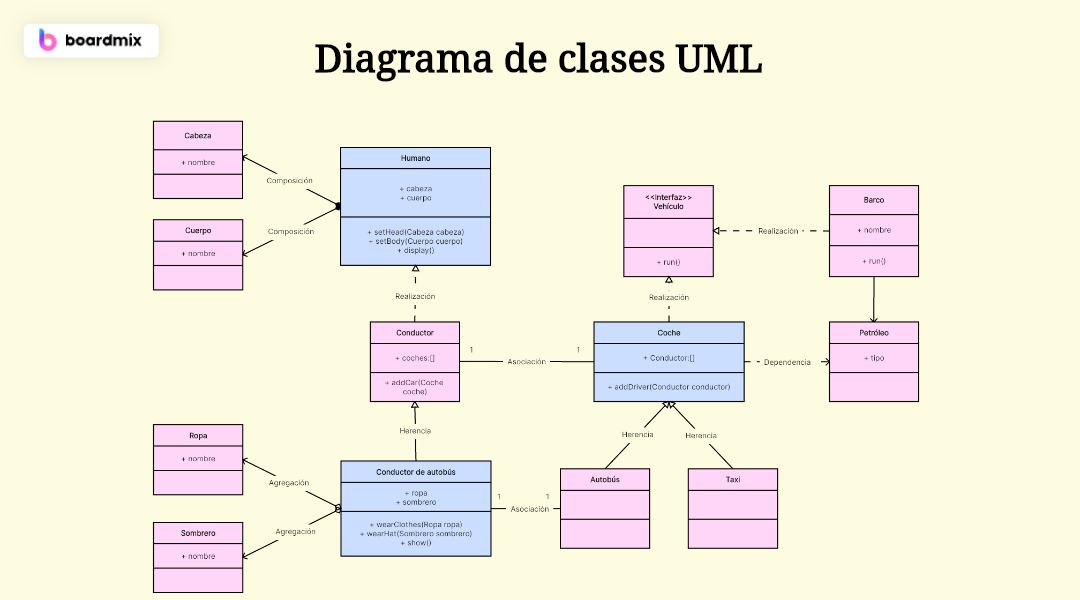
\includegraphics[width=0.8\textwidth]{Figures/diagrama-de-clases-uml.png}
    \caption*{Fonte: Autoria própria.}
    \label{fig:diagrama_classes}
\end{figure}

favor olhar a seção \ref{sec:class}.


\section{Diagrama de casos de uso}
\label{sec:casos}
O diagrama de casos de uso é uma representação visual dos casos de uso do sistema e os atores envolvidos. Ele é utilizado para descrever as funcionalidades do sistema e como os usuários interagem com ele. A Figura \ref{fig:diagrama_casos} apresenta o diagrama de casos de uso do sistema desenvolvido.

\section{Diagrama de sequência}
\label{sec:sequencia}   
O diagrama de sequência é uma representação visual da interação entre os objetos do sistema ao longo do tempo. Ele é utilizado para descrever como os objetos interagem entre si para realizar uma determinada funcionalidade. A Figura \ref{fig:diagrama_sequencia} apresenta o diagrama de sequência do sistema desenvolvido. 









    \include{Chapters/conclusao}
    % include more chapters ...
%
% ----------------------------------------------------------------------------
% Include thesis appendices
    \begin{thesisappendices}
        \include{Appendices/diagmec}
        \include{Appendices/diagele}
        %\include{Appendices/logbook}
    \end{thesisappendices}
%
% ----------------------------------------------------------------------------
% Configurar as referencias bibliograficas
	\renewcommand\bibname{Referências}
    \addcontentsline{toc}{chapter}{Referências}
    \bibliography{References/referencias}
%
% ----------------------------------------------------------------------------
% Finishing him
    \include{Others/ultimafolha}
\end{document}
%
% -------------------------------------------------------------------------------
% Aqui termina a formatação para o documento.
% In God We Trust. All Other Bring Data. 
%
% -------------------------------------------------------------------------------